
\documentclass[12pt]{report}

\usepackage{fullpage}
\usepackage{graphicx}
\usepackage{listings}
\usepackage{verbatim}
\usepackage{amsmath}
\usepackage{color}
\usepackage{hyperref}
 
\definecolor{codegreen}{rgb}{0,0.6,0}
\definecolor{codegray}{rgb}{0.5,0.5,0.5}
\definecolor{codepurple}{rgb}{0.58,0,0.82}
\definecolor{backcolour}{rgb}{0.95,0.95,0.92}
 
\lstdefinestyle{mystyle}{
    backgroundcolor=\color{backcolour},   
    commentstyle=\color{codegreen},
    keywordstyle=\color{magenta},
    numberstyle=\tiny\color{codegray},
    stringstyle=\color{codepurple},
    basicstyle=\footnotesize,
    breakatwhitespace=false,         
    breaklines=true,                 
    captionpos=b,                    
    keepspaces=true,                 
    numbers=left,                    
    numbersep=5pt,                  
    showspaces=false,                
    showstringspaces=false,
    showtabs=false,                  
    tabsize=2
}
 
\lstset{style=mystyle}
\renewcommand{\baselinestretch}{2}
\author{Mohammed Nauman Sididque}
\title{Comparision of Top 10 query results on Google and Bing }

\begin{document}
\maketitle
\tableofcontents

\chapter{Problem 1.1}
\section{Problem Statement}
Think up and write down a small number of queries for a web search engine.Make sure that the queries vary in length (i.e., they are not all one word). Try to specify exactly what information you are looking for in some of the queries. Run these queries on two commercial web search engines and compare the top 10 results for each query by doing relevance judgments. Write a report that answers at least the following questions: What is the precision of the results? What is the overlap between the results for the two search engines? Is one search engine clearly better than the other? If so, by how much? How do short queries perform compared to long queries?
\section{Query Results}

\subsection{Query 1: Manchester United}
The purpose of the query is to search relevant web pages about the soccer club Manchester United.
\subsubsection{Google Search Results}
Google search results for the query contain  Manchester United Twitter homepage link at the top search, two links to its official homepage followed by six links to news related to Manchester United.

\begin{figure}[ht]
  \centering
  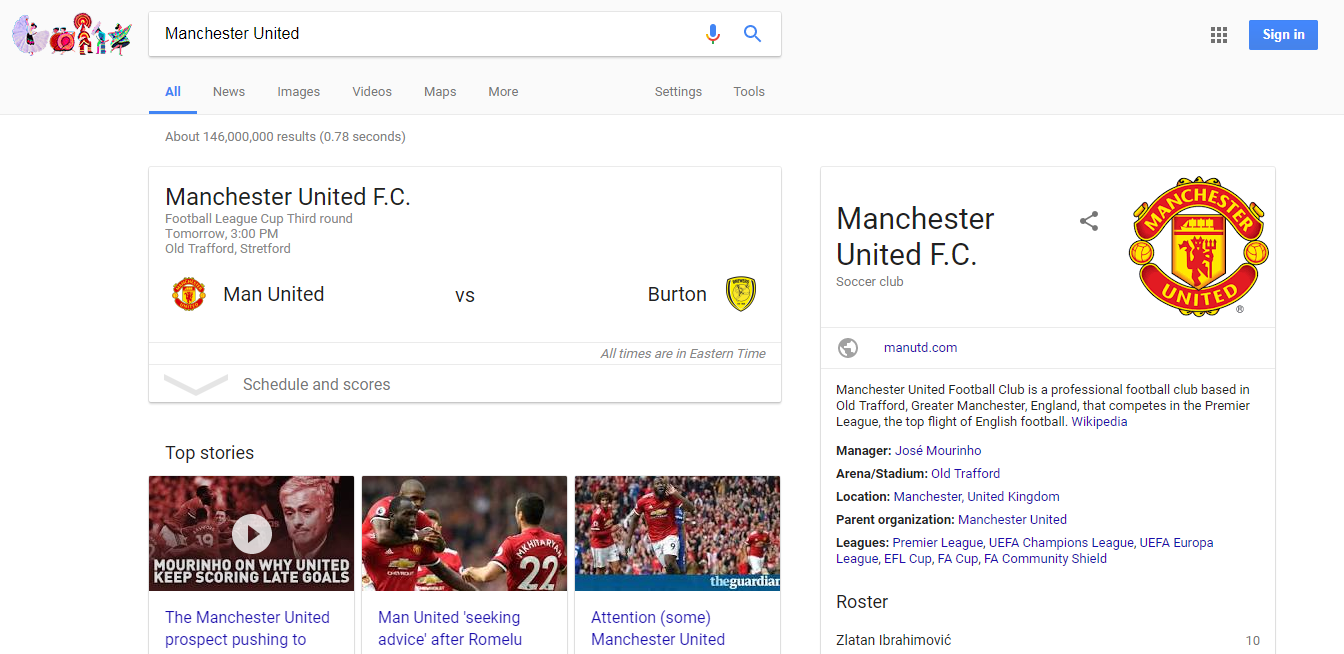
\includegraphics[width=0.7\textwidth]{Query1_Google.PNG}
  \caption{Google Search Results}
  \label{fig:1}
\end{figure}

\subsubsection{Bing Search Results}
Bing search results contain Manchester United official homepage as the top search followed by current news and videos relating to the club. Further, the result relates to other websites that host a page related to Manchester United. 

\begin{figure}[ht]
  \centering
  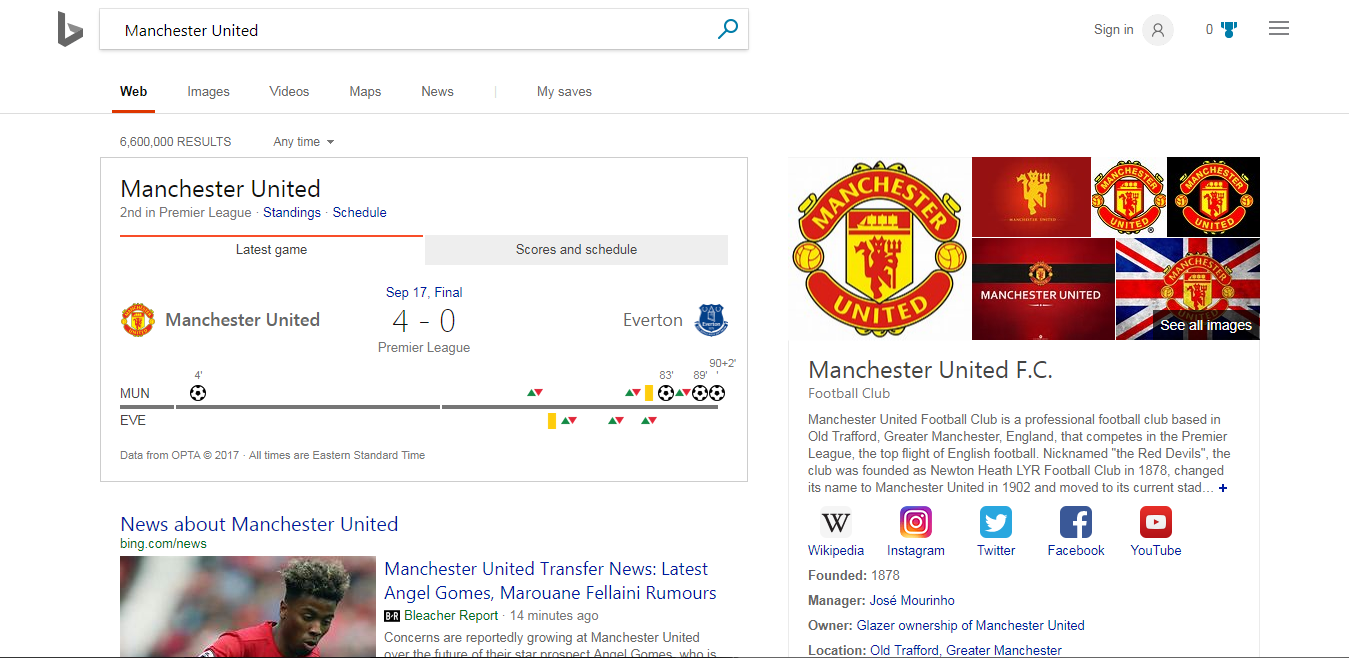
\includegraphics[width=0.7\textwidth]{Query1_Bing.PNG}
  \caption{Bing Search Results}
  \label{fig:2}
\end{figure}

\subsubsection{Better Results}
Bing contains more results on Manchester United club but Google search contains information relating to current news of the club in its search results. In my consideration, Google search results are on par with Bing search result.
\subsubsection{Overlap of Results}
Two search results overlap.

\subsection{Query 2: Mourinho stats Man Utd}
The purpose of this query is to find statistics of the current manager Jose Mourinho at the soccer club Manchester United.
\subsubsection{Google Search Results}
The search results contain two links which show statistics of the manager at the soccer club. One link is about the manager's Wikipedia page and rest other links are recent news articles relating to his current form and about his statistics at the soccer club.

\begin{figure}[ht] 
  \centering
  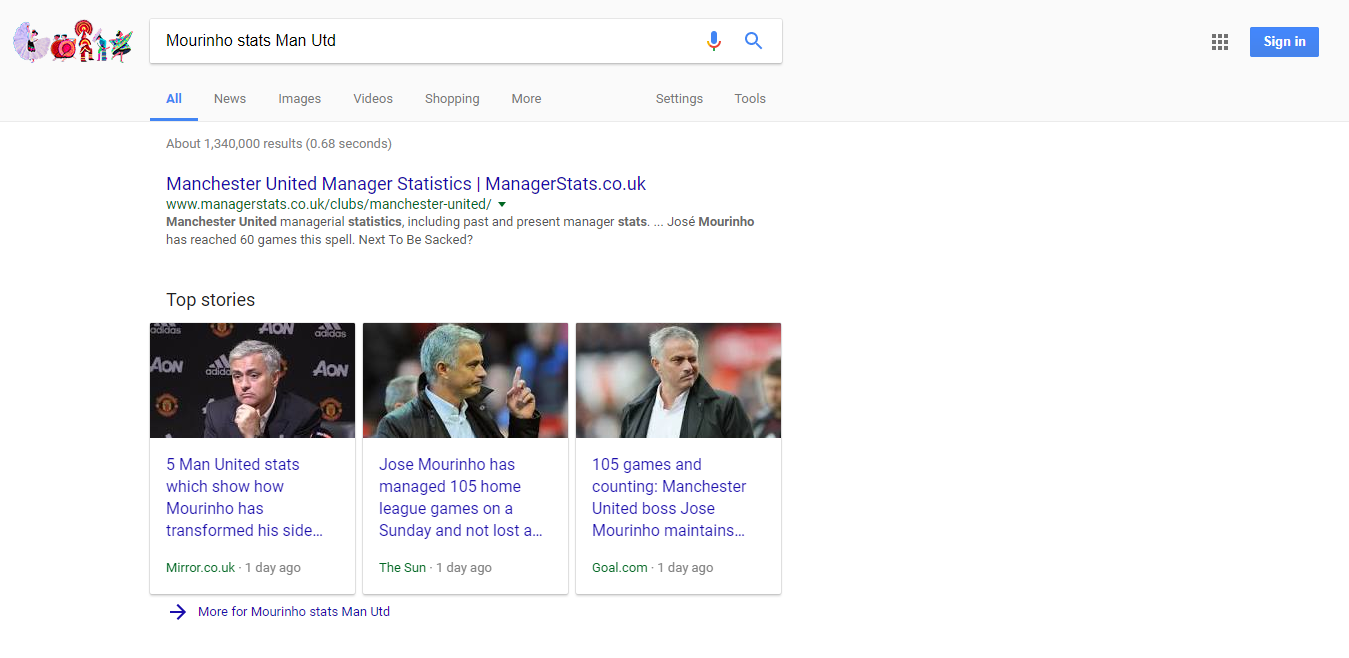
\includegraphics[width=0.7\textwidth]{Query2_Google.PNG}
  \caption{Google Search Results}
  \label{fig:3}
\end{figure}

\subsubsection{Bing Search Results}
The search results on Bing mainly revolve around current news and results relating to the soccer club.

\begin{figure}[ht]
  \centering
  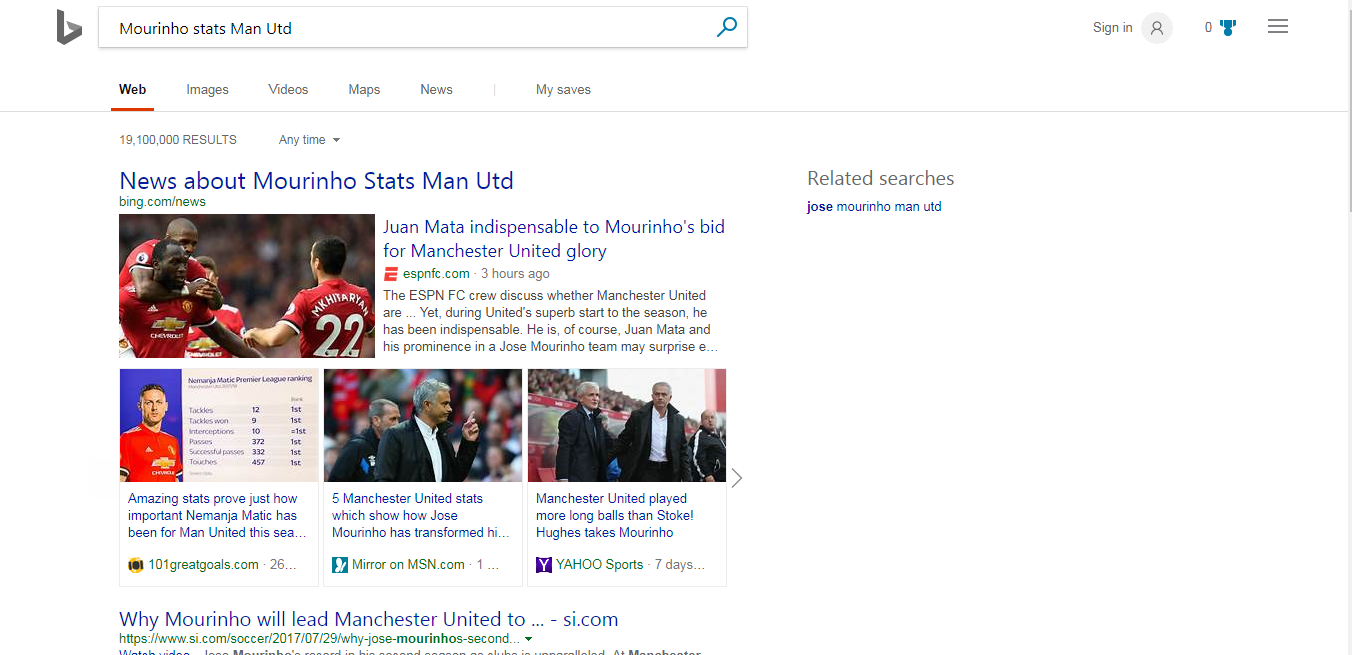
\includegraphics[width=0.7\textwidth]{Query2_Bing.PNG}
  \caption{Bing Search Results}
  \label{fig:4}
\end{figure}

\subsubsection{Better Results}
 Although Google has a couple of links to fulfill the requirements for this query, Bing search results are not relevant to the information seeker.
\subsubsection{Overlap of Results}
Zero search results overlap.

\subsection{Query 3: Ronaldo}
The purpose of this query is to search about Brazilian soccer legend Ronaldo, but it matches with the current soccer superstar Cristiano Ronaldo.
\subsubsection{Google Search Results}
The Google search result has a Wikipedia page of Brazilian superstar as its highest ranked page. But, the rest of the results revolve around current superstar Ronaldo which is not the desired search result. The last search result is a news article about Brazilian superstar Ronaldo.

\begin{figure}[ht]
  \centering
  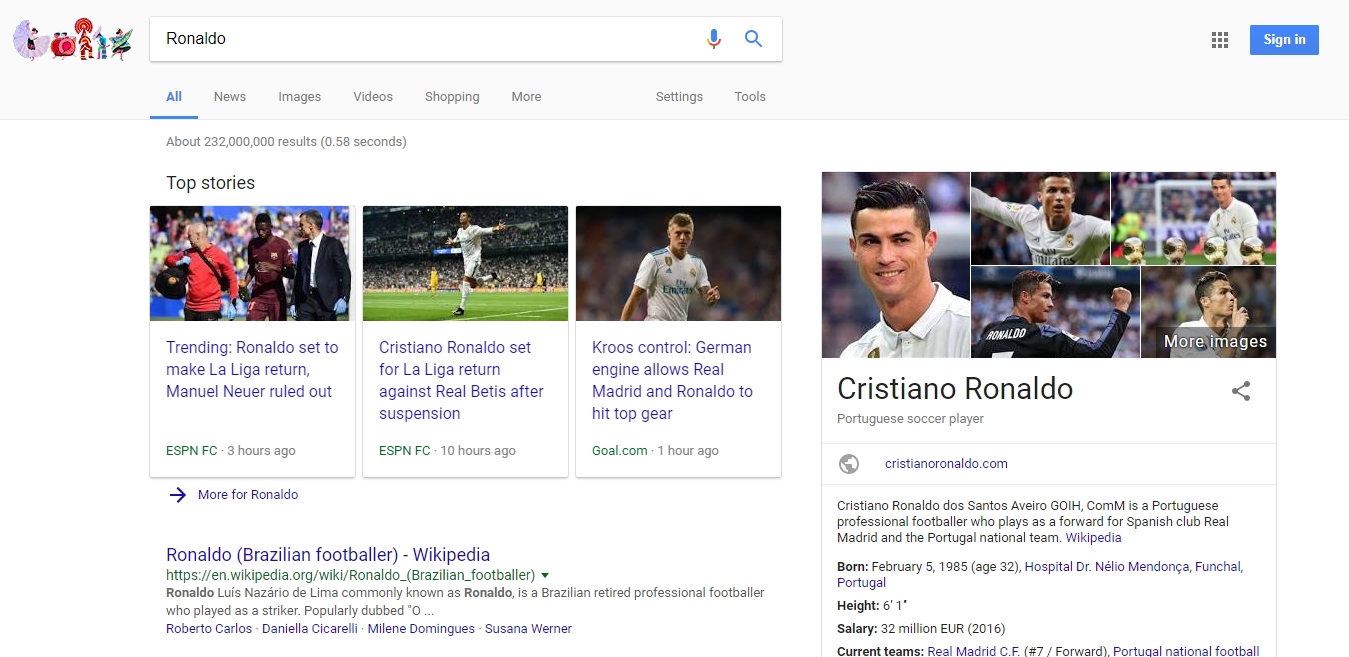
\includegraphics[width=0.7\textwidth]{Query3_Google.PNG}
  \caption{Google Search Results}
  \label{fig:5}
\end{figure}

\subsubsection{Bing Search Results}
The Bing search result indexes the current superstar Ronaldo. Further, it has a link about Ronaldo name significance and about a movie named Ronaldo. My query requirements are left unfullfilled.

\begin{figure}[ht]
  \centering
  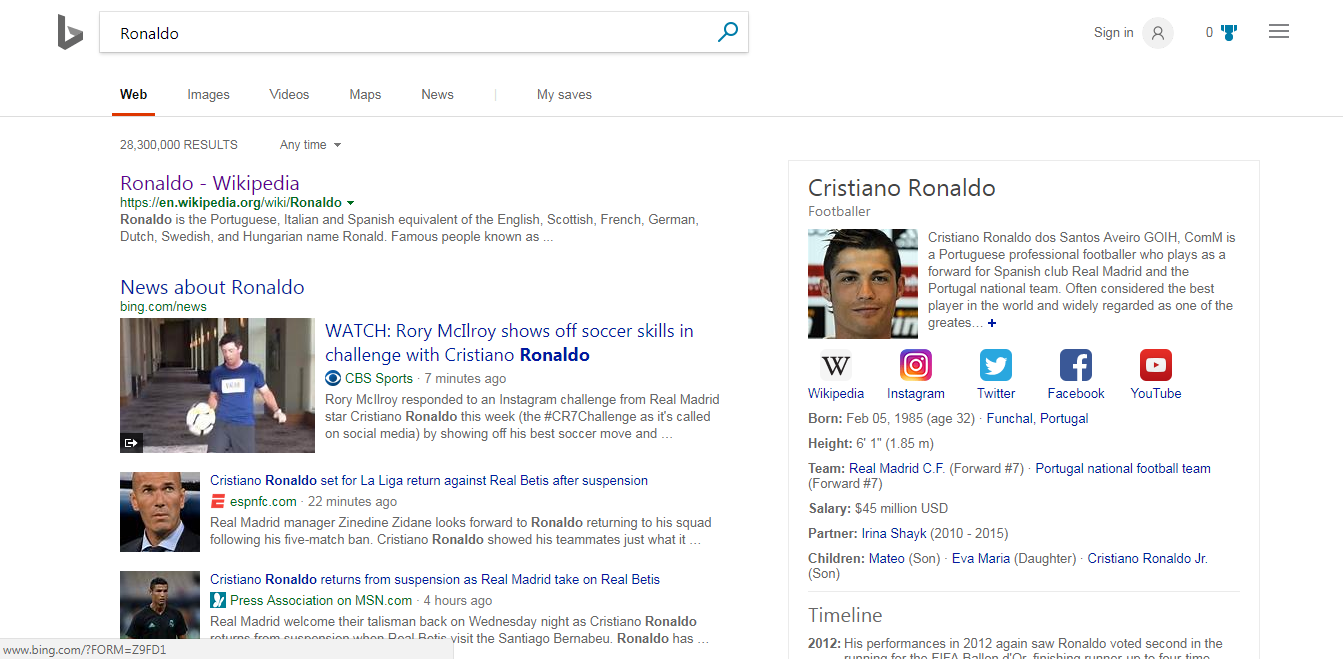
\includegraphics[width=0.7\textwidth]{Query3_Bing.PNG}
  \caption{Bing Search Results}
  \label{fig:6}
\end{figure}

\subsubsection{Better Search Results}
Although Google does not show many links relating to my query its results are more balanced than Bing which treats the football legend to be a lesser stature than the movie and even has a link to the understanding of name Ronaldo.
\subsubsection{Overlap of Results}
Four search results overlap.

\subsection{Query 4: Mohammed Nauman Siddique}
The purpose of the query is to find about myself.
\subsubsection{Google Search Results}
The highest ranked result on Google is a facebook profile which is not at all related to me. Further, it has my Linkedin profile and in later results Google dives in to find many other people that have name spelling as me.

\begin{figure}[ht]
  \centering
  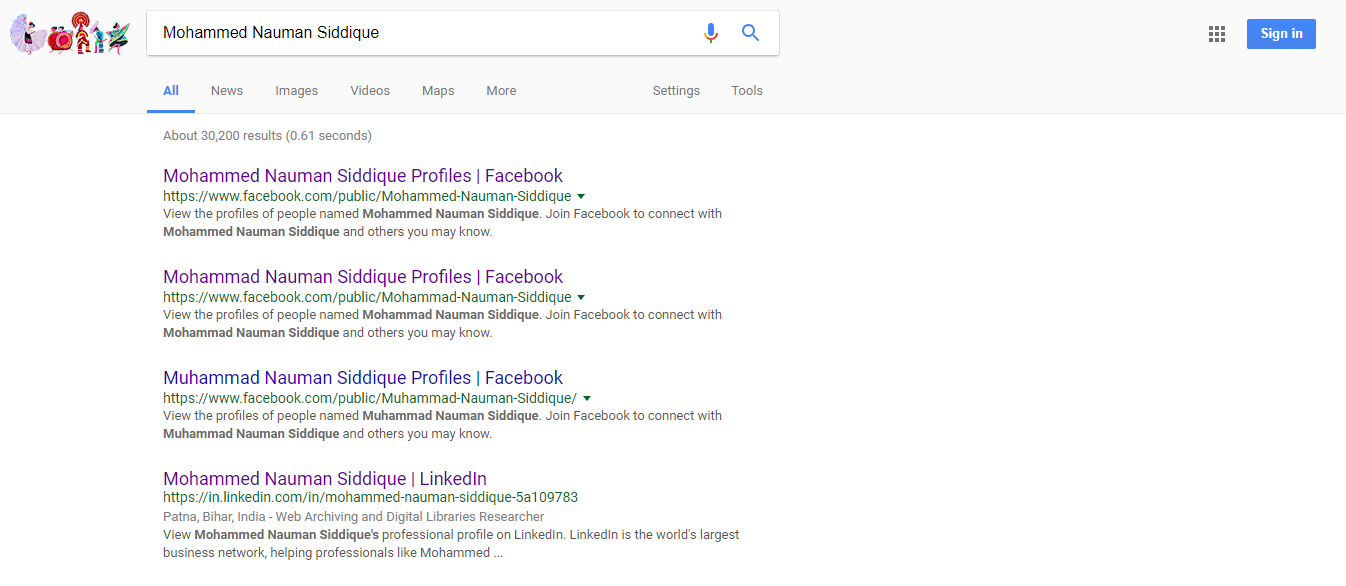
\includegraphics[width=0.7\textwidth]{Query4_Google.PNG}
  \caption{Google Search Results}
  \label{fig:7}
\end{figure}

\subsubsection{Bing Search Results}
The search results on Bing contain multiple links to my Linkedin profile but it also has results for another person with a similar name spelling.

\begin{figure}[ht]
  \centering 
  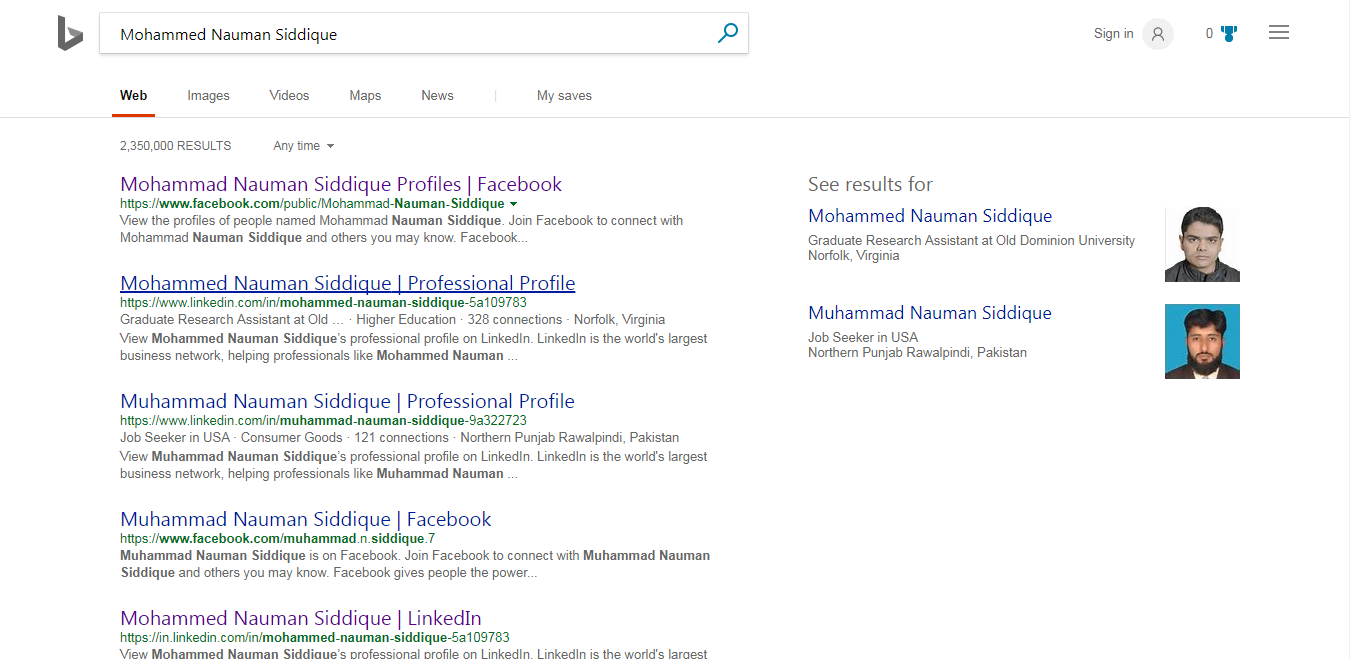
\includegraphics[width=0.7\textwidth]{Query4_Bing.PNG}
  \caption{Bing Search Results}
  \label{fig:8}
\end{figure}

\subsubsection{Better Search Results}
Bing ranked the most relevant document but Google could not do it. Although both of them did not link to any new web page. So, the results are equal for both.  
\subsubsection{Overlap of Results}
Five search results overlap.

\section{Conclusion}
In my query search results, Google comes out to be better than Bing for both long and short queries. Google tries to accommodate all sort of links, so you will eventually find your relevant link. While Bing search results are very streamlined. Once the highest ranked document is not the desired one, then better change your query because Bing will not fetch the desired links. I do not have any quantitative data to measure the search results of Google and Bing search results but qualitatively I will go for Google. 

\chapter{Problem 1.4}
\section{Problem Statement}
List five web services or sites that you use that appear to use search, not including web search engines. Describe the role of search for that service. Also describe whether the search is based on a database or grep style of matching, or if the search is using some type of ranking.
\section{Name of Web Services}
Amazon\\
Facebook\\
Twitter\\
Gmail\\
Wikipedia
\subsection{Amazon}
Amazon search is primarily about listing all the products available based on the keywords.The success of Amazon search depends on when you search a product and find it at a great price and buy it because you will return and buy more products. \cite{1} The search on Amazon is a database search model. \cite{2} Most of the e-commerce websites or product based sites maintain a catalog of their products in their databases. It becomes visible when we list our product onto Amazon. It demands the information in a specific format. So, you need data in a structured manner to fill their databases. Amazon does use ranking on its products. It is a keyword-based search engine which ranks its products based on price, availability, selection and sales history. \cite{1}

\subsection{Facebook}
Facebook search is about searching people, pages, places, check-ins, check-outs and objects with location information attached. In a nutshell, Facebook search replies to our natural language queries based on the previous data of its users and other user specific search results. It uses grep based search which is evident from the fact that it finds information from a user's network of events. The ranking of results is based on the content of the user their friends’ profiles and the relationships between the user and their friends. \cite{3}

\subsection{Twitter}
Twitter search can be used for searching tweets from yourself, friends, local businesses, and everyone from well-known entertainers to global political leaders. It also allows you to search for topic keywords or hashtags to follow any conversation of your interest. \cite{4} It is a grep based search which is evident from the functioning of the Twitter search engine.If we search for a keyword on Twitter, it lists all the tweets that contain those keywords. It provides us with an option to search tweets containing a particular keyword, hashtag, language, people, places, dates. \cite{5} It ranks the search results on the basis of your query input. It also has implemented a new feature of ranking the tweets you care about to be on the top of your timeline based on the accounts you interact the most. \cite{6}

\begin{figure}[ht]
  \centering
  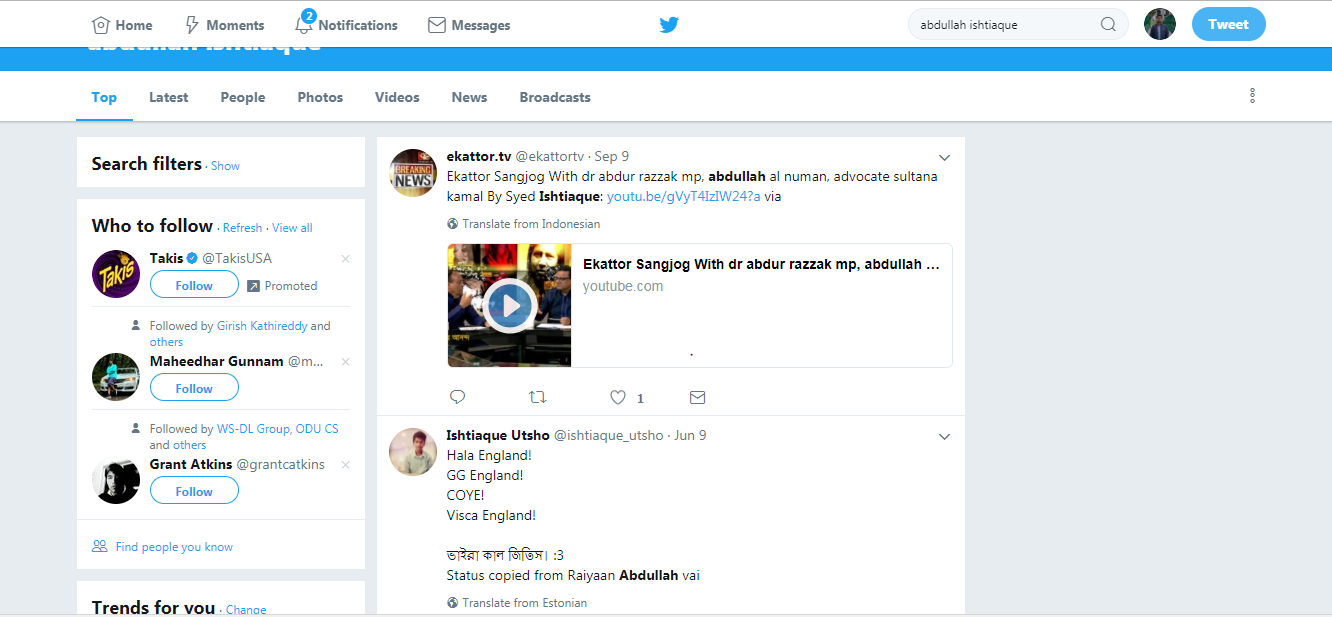
\includegraphics[width=0.7\textwidth,]{TwitterSearch.PNG}
  \caption{Twitter Search }
  \label{fig:9}
\end{figure}

\subsection{Gmail}
Gmail search can be used to search for emails containing the keywords typed in the search box. It has a grep based search result which is evident as it displays only the emails that contain the keywords typed in the search box. It ranks the emails on the basis of date and keywords in the e-mail. 

\begin{figure}[ht]
  \centering
  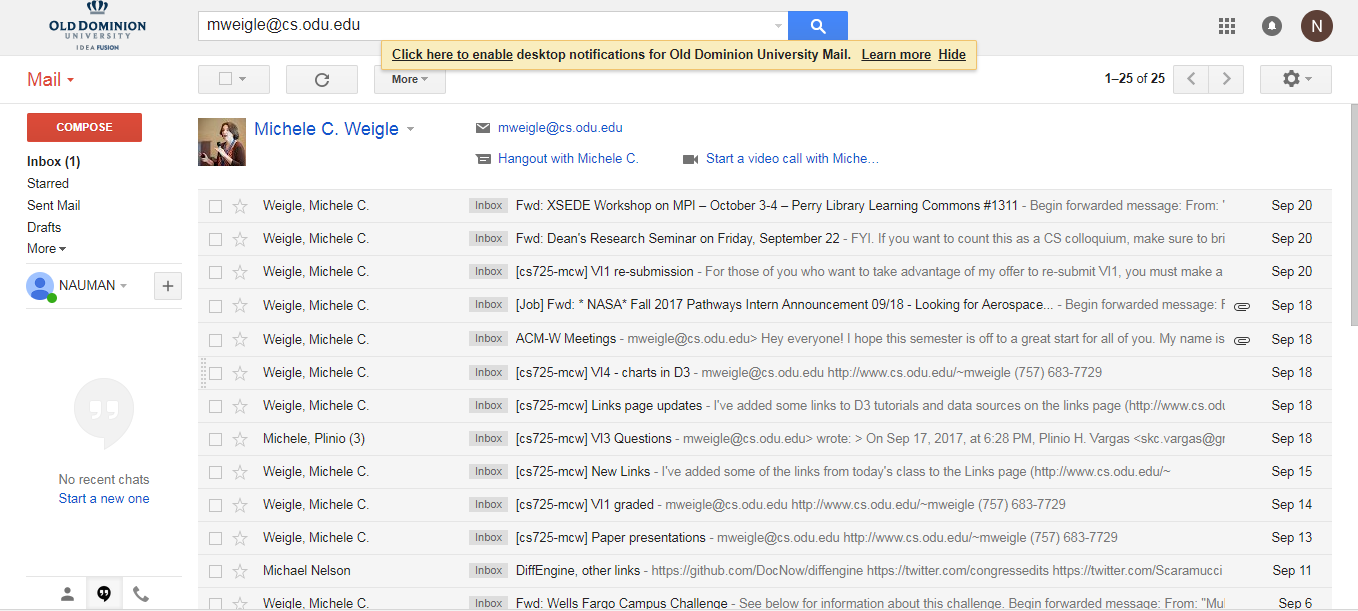
\includegraphics[width=0.7\textwidth,]{GmailSearch.PNG}
  \caption{Gmail Search }
  \label{fig:10}
\end{figure}

\subsection{Wikipedia}
Wikipedia is an encyclopedia for information. \cite{7} It has a database search mechanism. It becomes apparent when an unknown keyword is typed, it does not list any results but it might give some suggestions. The ranking of Wikipedia search results depends on a number of factors with the number of links to an article being one of them. \cite{8}

\begin{figure}[ht]
  \centering
  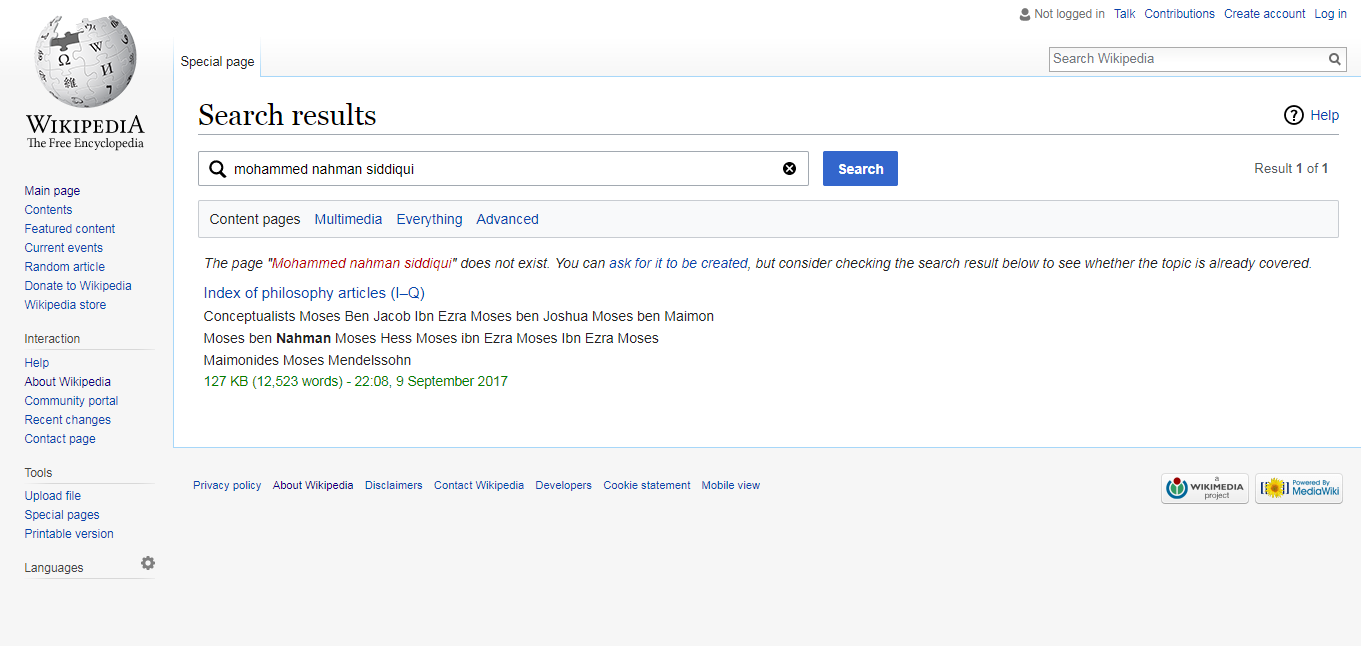
\includegraphics[width=0.7\textwidth,]{Wikipedia_Search.PNG}
  \caption{Wikipedia Search Results}
  \label{fig:11}
\end{figure}

\chapter{Problem 3.7}
\section{Problem Statement}
Write a program that can create a valid sitemap based on the contents of a directory on your computer’s hard disk. Assume that the files are accessible from a website at the URL http://www.example.com. For instance, if there is a file in your directory called homework.pdf, this would be available at http://www.example.com/homework.pdf. Use the real modification date on the file as the last modified time in the sitemap, and to help estimate the change frequency.
\section{Sitemap Generation Code}
\lstinputlisting[language=Python]{TestSitemap.py}
\section{Code Description}
The code is about generating sitemap XML for the url provided to the code. It searches for a set of file extension i.e .pdf, .css, .html and .png. \cite{9} The file extension was used for listing to filter the sitemaps generation because we wanted only a subset of files to be visible on our sitemap. It lists the URL of the file, last modified time and change frequency in the XML. Change frequency parameter is calculated on the basis of difference between the current UTC time (i.e when this file was initially generated) and the last modified time. 
\subsection{Limitations of the Code}
This code does not contain the correct value of change frequency. We can get the file creation time for Windows but Linux does not provide the file creation time. \cite{10} If the file creation date was available we could have tried to check for the difference with its modified time and then we would have two difference value (one difference is already calculated in the current implementation) to get our change frequency value.  
\section{Output of the code}

\begin{figure}[ht]
  \centering
  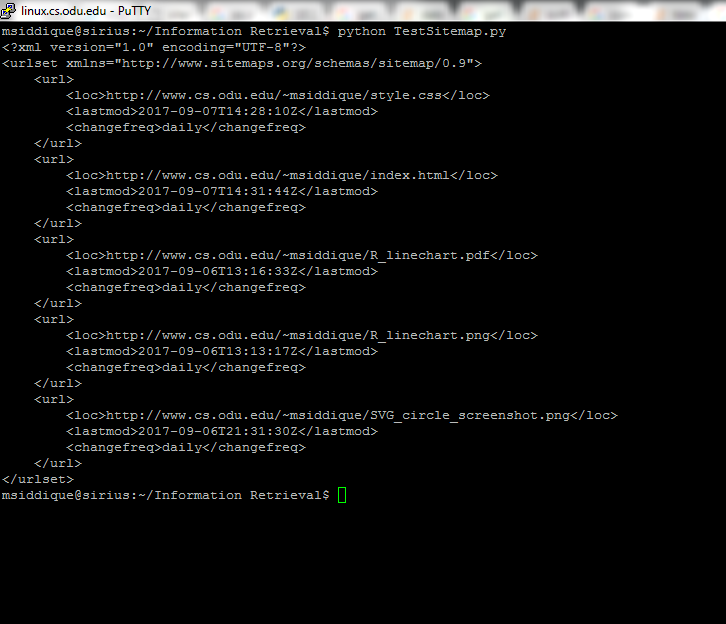
\includegraphics[width=0.7\textwidth,]{Sitemap_Output.PNG}
  \caption{Sitemap Output}
  \label{fig:10}
\end{figure}

\chapter{Problem 3.8}
\section{Problem Statement}
Suppose that, in an effort to crawl web pages faster, you set up two crawling machines with different starting seed URLs. Is this an effective strategy for distributed crawling? Why or why not?
\section{Distributed Crawling on seed URLs}
The web is too enormous for a single crawler to crawl. Therefore we use a distributed approach for crawling. The advantages to distributed crawling over a single machine crawling as follows:\\
Easy to crawl nearby websites\\
Number of sites the crawler has to remember\\
Increased Computation Power\\
One of the ways to set up our crawler for the distributed approach is to provide each crawler a list of seed URLs to crawl on. 
\subsection{Easy to crawl nearby websites}
 A crawler can crawl a geographically closer website at a faster rate compared to a website that is farther away in geographical location. A crawler makes a request to web server for content of its web pages and receives the content in return from the web server. Long distance network communications have a lower throughput due to increased latency in data communication. We can exploit the distributed crawling by  provided seeded URLs based on their geographical location to  the two crawling machines.
\subsection{Number of sites the crawler has to remember}
A crawler always has to maintain a list of URLs it has already crawled over, in order to crawl them again for freshness. Furthermore, every time a new URL is crawled the crawler fetches a number of URLs from its content. These URLs are checked against its current queue and added to the search queue if it turns to be a new URL. Therefore crawling with seeded URLs means it has to be concerned about the  lesser number of URLs and reduces the chances of crawling over duplicate URLs.
\subsection{Increased Computation Power}
Two crawling machines are better than a single crawling machine due to their increased CPU resources and network bandwidth. In respect to seeded URLs, each machine has to be concerned with a lesser number of URL, so more time is spent on crawling new pages rather than maintaining its own internal crawling system.
\subsection{Disadvantages of seeded URL approach}
It might happen that a crawling machine has a popular website in its seeded URL to crawl over. So, it could arise that one of the machines has to crawl more than the other. But this issue can be fixed by load balancing mechanism. 
\chapter{Problem 3.9}
\section{Problem Statement}
Write a simple single-threaded web crawler. Starting from a single input URL (perhaps a professor’s web page), the crawler should download a page and then wait at least five seconds before downloading the next page. Your program should find other pages to crawl by parsing link tags found in previously crawled documents.
\section{Web Crawler Code}
\lstinputlisting[language=Python]{Crawler.py}
\section{Code Description}
The code on Web Crawler starts its crawl from URL `http://www.cs.odu.edu/~mln/' and download the HTML contents and save them to a file. The HTML content is further parsed to get URL links and added to the list of URIs to be parsed. The crawling process works till the list of URIs become empty.A politness window of 5 seconds has been implemented in the crawler to stop it from sending continuous requests to the web server. Beautiful Soup library has been used to parse through the HTML to retrieve URIs from the HTML content.  \cite{11} The code was run for a few minutes to test for its output, so the output might not be as exhaustive as expected.  
\section{Output}
The results of URI are in the last chapter of the assignment report.
\begin{figure}[ht]

  \centering
  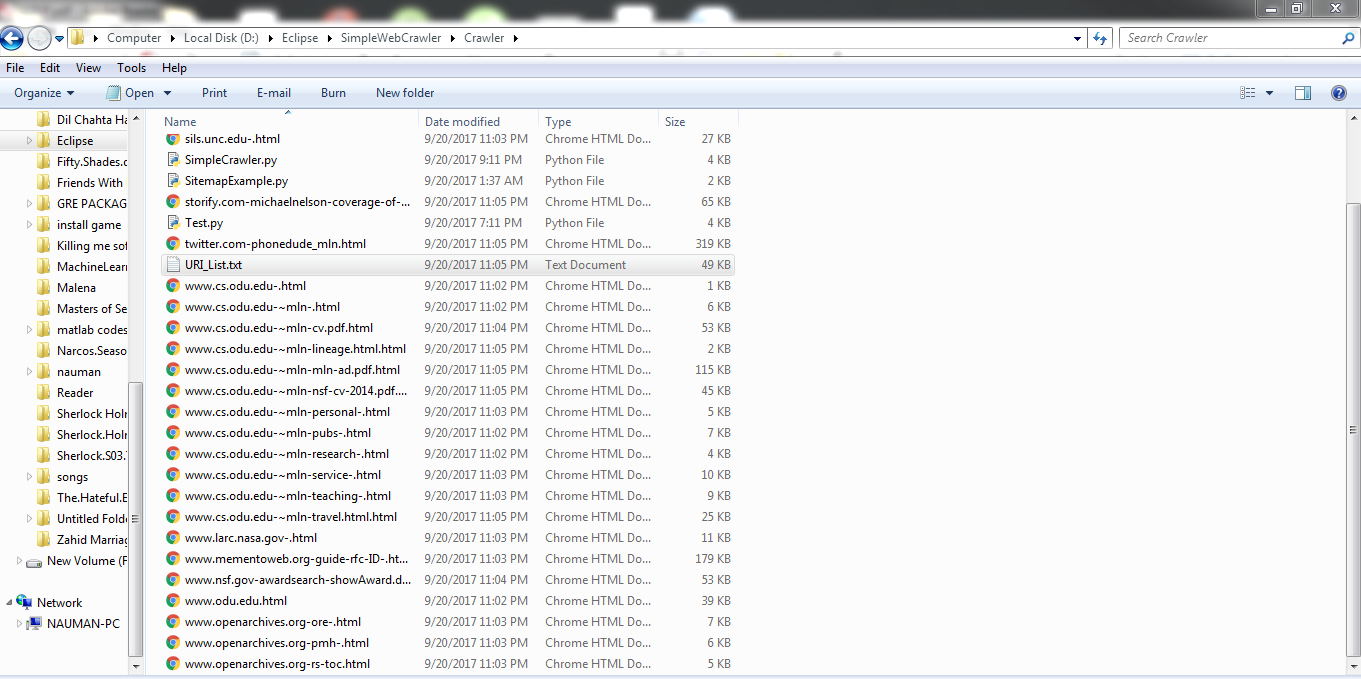
\includegraphics[width=0.7\textwidth,]{Crawl.PNG}
  \caption{Screenshot of Crawled Pages}
  \label{fig:11}
\end{figure}

\begin{thebibliography}{9}
\bibitem{1}
 Grimm, Nathan. `How to Rank Well in Amazon, the US's Largest Product Search Engine', 2014 [Online], \url{ https://moz.com/blog/amazon-seo-organic-search-ranking-factors} [Accessed: 09/19/2017] 
\bibitem{2}
Amazon. `What Is Amazon Relational Database Service (Amazon RDS)?', 2014[Online],\url{ http://docs.aws.amazon.com/AmazonRDS/latest/UserGuide/Welcome.html} [Accessed: 09/19/2017]
\bibitem{3}
Wikipedia. `Facebook Graph Search', 2013[Online], \url{https://en.wikipedia.org/wiki/Facebook_Graph_Search/} [Accessed: 09/19/2017]
\bibitem{4}
Twitter. `Using Twitter search', \url{https://support.twitter.com/articles/132700} [Accessed:09/19/2017] 
\bibitem{5}
Twitter. `Using advanced search', \url{https://support.twitter.com/articles/71577} [Accessed:09/19/2017] 
\bibitem{6}
Twitter. `About your Twitter timelineh', \url{https://support.twitter.com/articles/164083} [Accessed:09/19/2017] 
\bibitem{7}
Wikipedia. `Wikipedia:Introduction', 2004[Online], \url{https://en.wikipedia.org/wiki/Wikipedia:Introduction} [Accessed: 09/19/2017]
\bibitem{8}
Wikipedia. `Wikipedia:Wikipedia Signpost/2008-11-10/Search engine', 2008[Online], \url{https://en.wikipedia.org/wiki/Wikipedia:Wikipedia_Signpost/2008-11-10/Search_engine} [Accessed: 09/19/2017]
\bibitem{9}
Cook, John D.  `Code to make an XML sitemap', 2008[Online], \url{https://www.johndcook.com/blog/2008/02/25/code-to-make-an-xml-sitemap/} [Accessed: 09/19/2017]
\bibitem{10}
stackoverflow, `How to get file creation \& modification date/times in Python?', \url{https://stackoverflow.com/questions/237079/how-to-get-file-creation-modification-date-times-in-python} [Accessed: 09/19/2017]
\bibitem{11}
Beautiful Soup. `Beautiful Soup Documentation', \url{ https://www.crummy.com/software/BeautifulSoup/bs4/doc/} [Accessed: 09/20/2017]
\end{thebibliography}

\chapter{URI Results from Crawls}
\verbatiminput{URI_List.txt} 

\end{document}